\documentclass[11pt,letterpaper]{article}

% ====== Packages ======
\usepackage[margin=1in]{geometry}
\usepackage{times}
\usepackage{hyperref}
\usepackage{graphicx}
\usepackage{enumitem}
\usepackage{titlesec}

% ====== Formatting overrides ======
\titleformat{\section}{\large\bfseries}{\thesection.}{0.5em}{}
\setlength{\parindent}{0pt}
\setlength{\parskip}{0.5em}

% ====== Title and Header ======
\title{\vspace{-1.5cm}\textbf{CS543/ECE549 Project Progress Report}}
\author{\textbf{Yanjun Qin} \and \textbf{Hongbin Yang}}
\date{}

\begin{document}

\maketitle
\vspace{-2cm} 

% =========================================================
\section*{1. Updated Statement of Project Definition and Goals}
% =========================================================
Our core objective remains unchanged: to develop a robust automated system for detecting and quantifying surface defects on fruits (e.g., bruises/rots/scabs) for quality grading. Our minimum goal is to implement (i) a traditional Computer Vision (CV) baseline for binary defect segmentation and (ii) a Vision Transformer (ViT) pipeline for 4-class disease classification. Our maximum goal is to (i) interpret model behavior via attention visualization and (ii) implement a unified grading logic (Premium / Grade I / Reject) that integrates defect area ratio and class prediction.

\textbf{Update since proposal:} We have completed the end-to-end ViT training pipeline and initial attention rollout visualizations, and we have implemented multiple CV segmentation variants with quantitative IoU evaluation on a manually annotated subset. No scope changes were made; rather, the progress confirms that the classical baseline is sensitive to lighting artifacts, motivating deeper analysis and robustness improvements.

% =========================================================
\section*{2. Current Member Roles and Collaboration Strategy}
% =========================================================
\begin{itemize}[noitemsep, topsep=0pt]
    \item \textbf{Hongbin Yang:} Traditional CV pipeline (HSV thresholding + morphology) and segmentation evaluation. Responsible for dataset preprocessing, mask annotation workflow (LabelMe), and IoU evaluation on the manually annotated subset.
    \item \textbf{Yanjun Qin:} Deep learning pipeline (ViT fine-tuning) including data formatting for transformer inputs, training/evaluation scripts, and attention rollout visualization for interpretability.
\end{itemize}
\textit{Collaboration:} We use GitHub for code versioning and shared experiment artifacts. We hold a weekly synchronization meeting (Saturday) to review results and decide next experiments. We maintain a fixed dataset split (Train/Test) to avoid data leakage, and keep a dedicated folder (\texttt{mark\_pic/}) for image--mask pairs used in segmentation evaluation.

% =========================================================
\section*{3. Proposed Approach}
% =========================================================
As outlined in our proposal, we develop two complementary pipelines and compare them under a unified evaluation protocol.

\textbf{(A) Traditional CV pipeline (binary defect segmentation):} Implemented in Python using OpenCV [1]. The segmentation is defined at pixel level (Healthy vs. Defective). Our baseline steps are:
\begin{enumerate}[noitemsep, topsep=0pt]
    \item \textbf{Color Space Conversion:} Convert input BGR images to the HSV color space to decouple intensity from color information.
    \item \textbf{Thresholding:} Apply hard-coded HSV bounds to isolate potential defect areas (e.g., darker regions for Rot and Scab).
    \item \textbf{Morphological Noise Reduction:} Apply a Morphological Opening operation (using a 5x5 kernel) to remove isolated background noise, followed by a Closing operation to fill small holes within the segmented defect regions.
\end{enumerate}
To address the key limitation in our proposal (lighting sensitivity), we also implemented two robustness-motivated variants: (i) adaptive thresholding on the V channel with CLAHE contrast normalization, and (ii) watershed-based refinement. These variants are evaluated with the same IoU protocol.

\textbf{(B) ViT pipeline (4-class classification):} We fine-tune a pre-trained Vision Transformer (ViT-Base, Patch-16) [2] using transfer learning. The pipeline is:
\begin{enumerate}[noitemsep, topsep=0pt]
    \item \textbf{Preprocessing:} resize to $224\times 224$ and apply train-time augmentation (rotation, color jitter, random erasing).
    \item \textbf{Model:} ViT encoder + classification head for 4 classes (Normal/Blotch/Rot/Scab).
    \item \textbf{Training:} optimize cross-entropy with cosine LR schedule and warmup; mitigate imbalance via WeightedRandomSampler and class weights.
    \item \textbf{Evaluation:} report Accuracy, macro-F1, and a confusion matrix on the held-out test split.
    \item \textbf{Interpretability:} compute attention rollout maps [3] to visualize which image regions contribute most to the [CLS] token aggregation.
\end{enumerate}

\textbf{Planned integration (grading):} Our maximum-goal grading system will combine (i) defect area ratio from the CV segmentation mask and (ii) the ViT class prediction to produce a final grade (Premium / Grade I / Reject). This integration and its evaluation remain in progress.

% =========================================================
\section*{4. Data}
% =========================================================
We are utilizing the publicly available \href{https://www.kaggle.com/datasets/kaivalyashah/apple-disease-detection}{Apple Fruit Disease Dataset} from Kaggle. The data collection process is complete. The dataset has been rigorously split to prevent data leakage:
\begin{itemize}[noitemsep, topsep=0pt]
    \item \textbf{Training Set (386 images):} Blotch (117), Normal (68), Rot (115), Scab (86).
    \item \textbf{Testing Set:} Maintained separately for final evaluation.
\end{itemize}
\textbf{Annotations:} For pixel-level evaluation of the CV segmentation pipeline, we manually annotated a subset of test images using LabelMe to create binary masks (Healthy vs. Defective). We planned 50 images (15 per defect class and 5 Normal as a control group for false positives); at the time of this report, \textbf{40 image--mask pairs} are available in our evaluation folder and are used for quantitative IoU benchmarking.

% =========================================================
\section*{5. Initial Results}
% =========================================================
We have successfully implemented the initial CV steps and the evaluation metrics. We ran our baseline script across the 50 manually annotated Ground Truth masks. The baseline achieved a \textbf{Mean Intersection over Union (mIoU) of 0.2682}. 

Below is an illustration of the intermediate stages of our approach, demonstrating the transition from the original image to the raw HSV mask, and finally to the morphologically cleaned mask.

\begin{figure}[h]
    \centering
    % REPLACE 'figure_1.png' WITH THE ACTUAL FILENAME UPLOADED TO OVERLEAF
    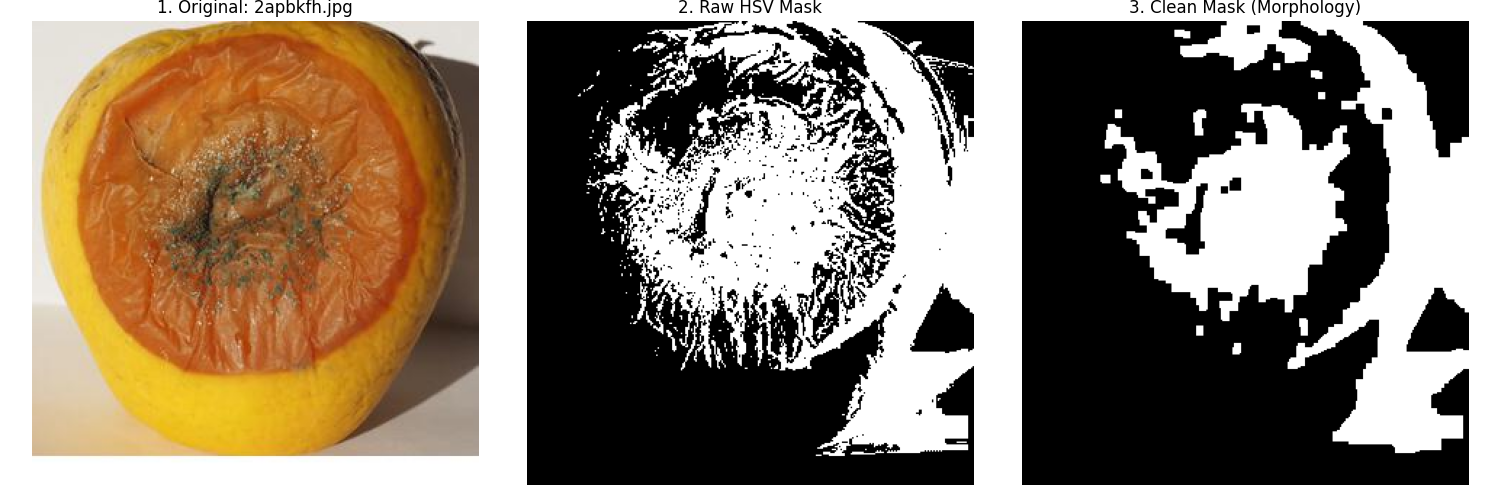
\includegraphics[width=0.9\textwidth]{figure_1.png}
    \caption{Intermediate stages of the Traditional CV Pipeline. Left: Original Image. Middle: Raw HSV Mask. Right: Clean Mask after Morphological Opening and Closing.}
\end{figure}

\vspace{0.5em}
\textbf{ViT classification (completed):} We successfully ran a full end-to-end training experiment for the Vision Transformer (ViT) pipeline for 4-class disease classification. We fine-tuned a \textbf{ViT-Base} model (Patch-16, input resolution $224\times 224$) using transfer learning. To mitigate class imbalance, we used a \textbf{WeightedRandomSampler} and inverse-frequency \textbf{class weights}. We also applied aggressive data augmentation (random rotation, color jitter, random erasing) to reduce overfitting on the limited dataset.

\textbf{Experiment configuration (vit\_base\_run):}
\begin{itemize}[noitemsep, topsep=0pt]
    \item \textbf{Train / Test split:} 382 training images, 120 test images.
    \item \textbf{Hyperparameters:} epochs=30 (early-stopped at epoch 28), batch size=16, lr=$2\times 10^{-5}$, weight decay=$1\times 10^{-4}$, warmup=3 epochs, seed=42.
    \item \textbf{Best checkpoint:} epoch 20 with \textbf{val\_acc=0.9000} and \textbf{val\_macro-F1=0.8935}.
\end{itemize}

\begin{figure}[h]
    \centering
    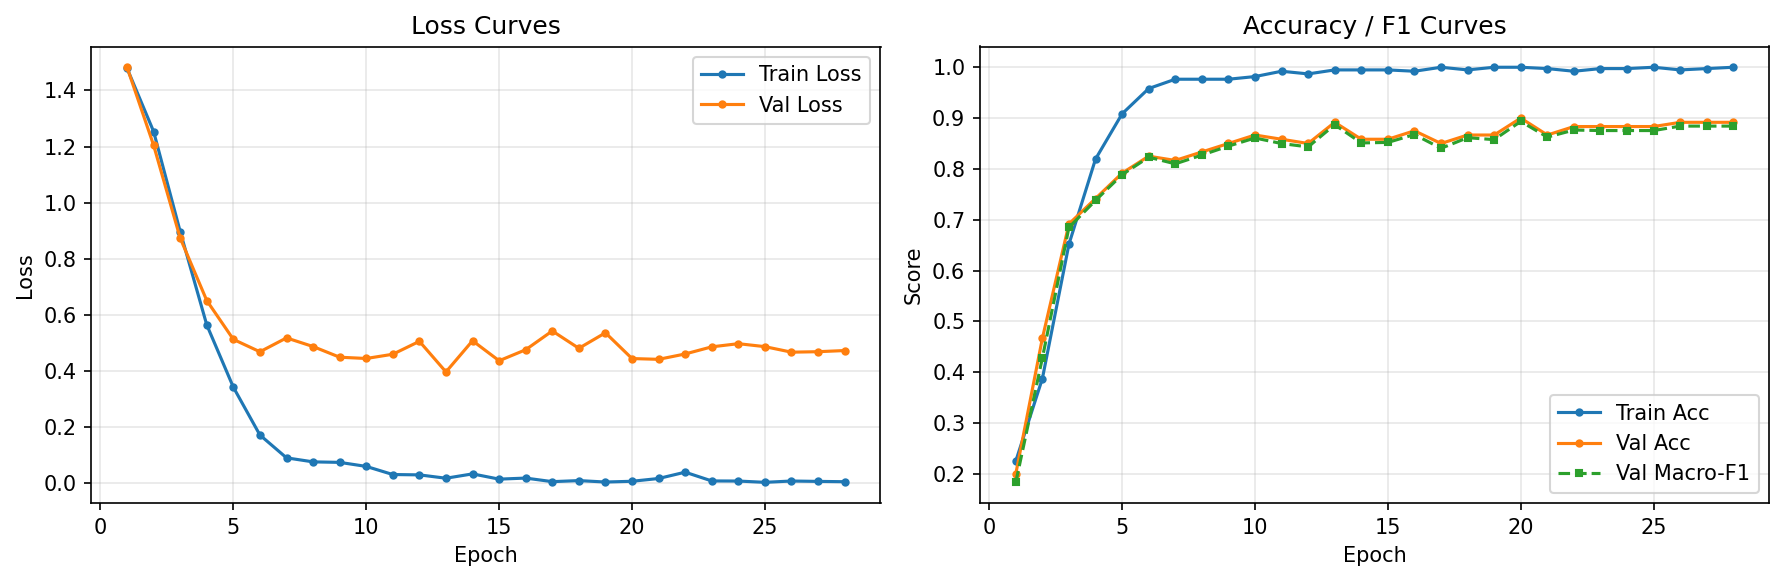
\includegraphics[width=0.95\textwidth]{training_curves.png}
    \caption{Training curves for the ViT pipeline (\texttt{vit\_base\_run}). Early stopping was triggered after epoch 28 with best validation accuracy at epoch 20.}
\end{figure}

\begin{figure}[h]
    \centering
    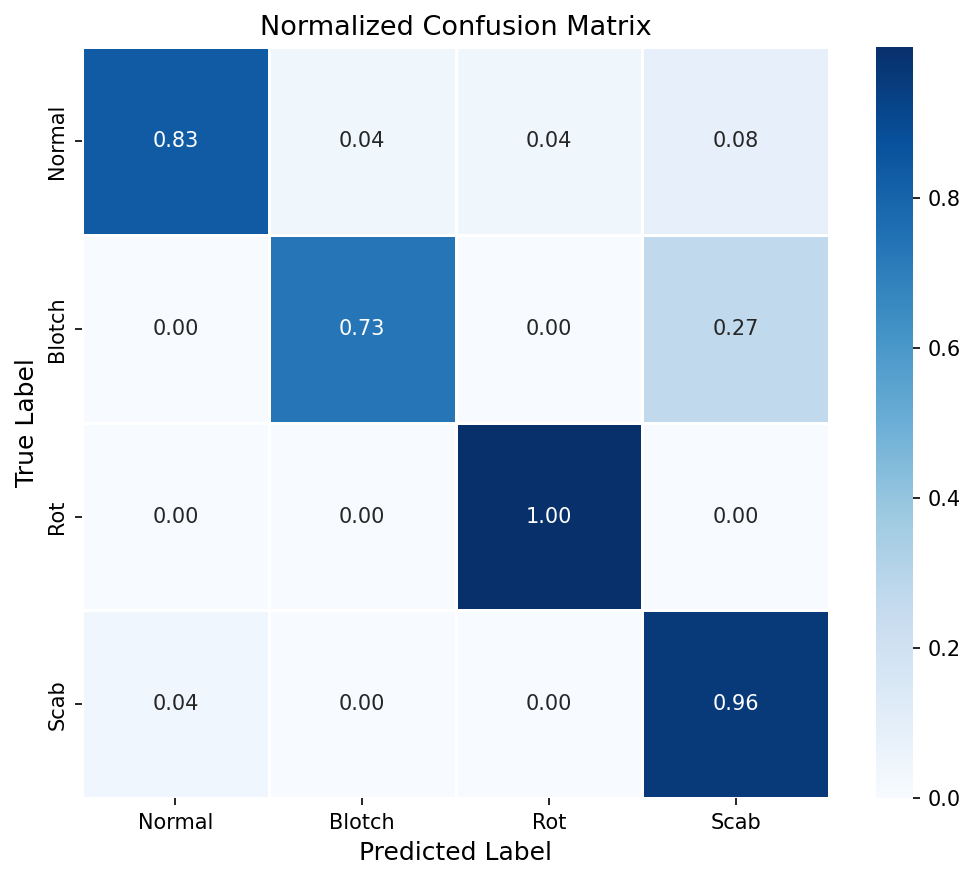
\includegraphics[width=0.75\textwidth]{confusion_matrix.png}
    \caption{Confusion matrix on the held-out test split for the ViT pipeline (\texttt{vit\_base\_run}).}
\end{figure}

\vspace{0.5em}
\textbf{Attention rollout visualization (completed):} To interpret our ViT's decision-making process, we generated attention rollout visualizations (Abnar \& Zuidema, 2020) using our best checkpoint. We curated 12 representative test images including both strong successes and notable failures (often under challenging lighting, such as shadows or specular highlights). Each visualization contains three panels: original image, attention heatmap, and an overlay. A CSV manifest recording \texttt{(image, true label, predicted label, confidence)} is included for reproducibility.

\begin{figure}[h]
    \centering
    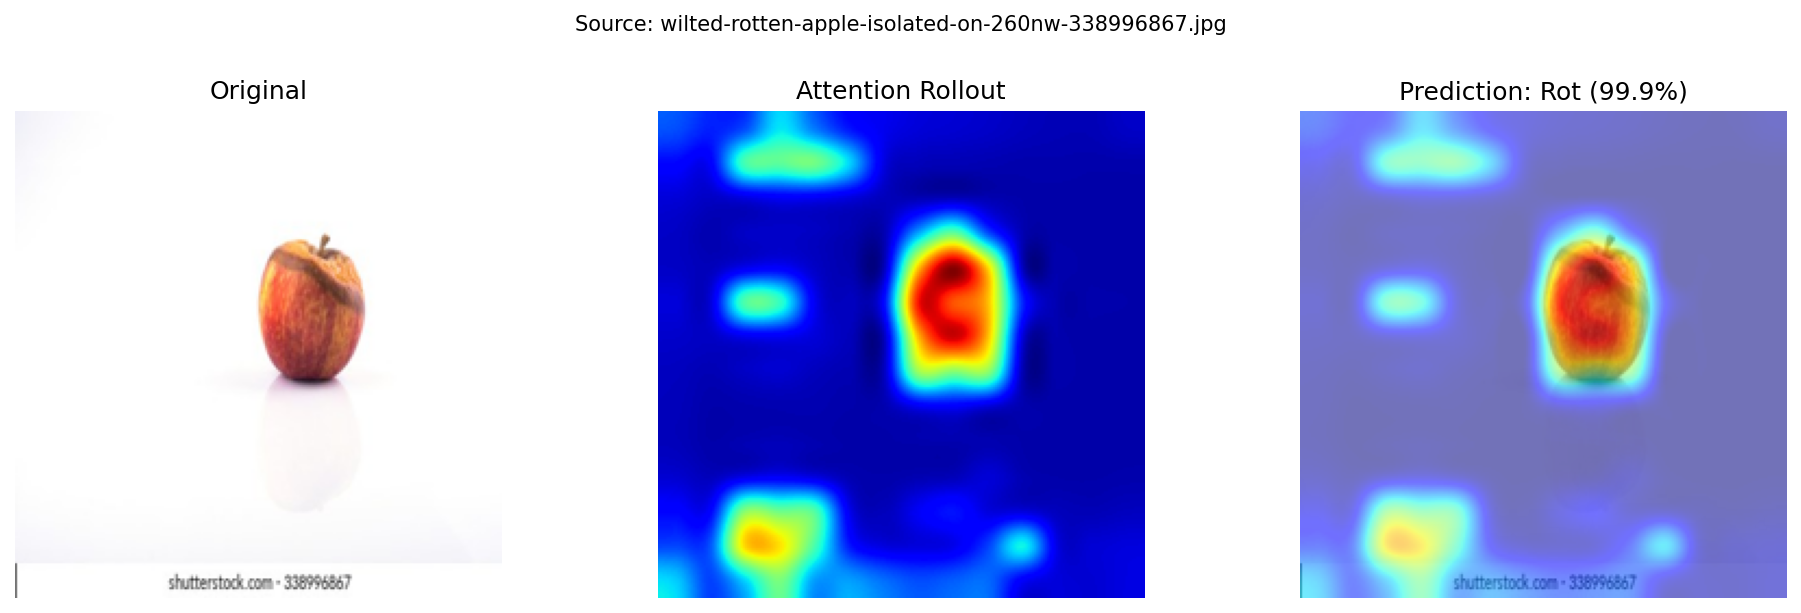
\includegraphics[width=0.95\textwidth]{attn_good_correct_24.png}
    \vspace{0.2em}
    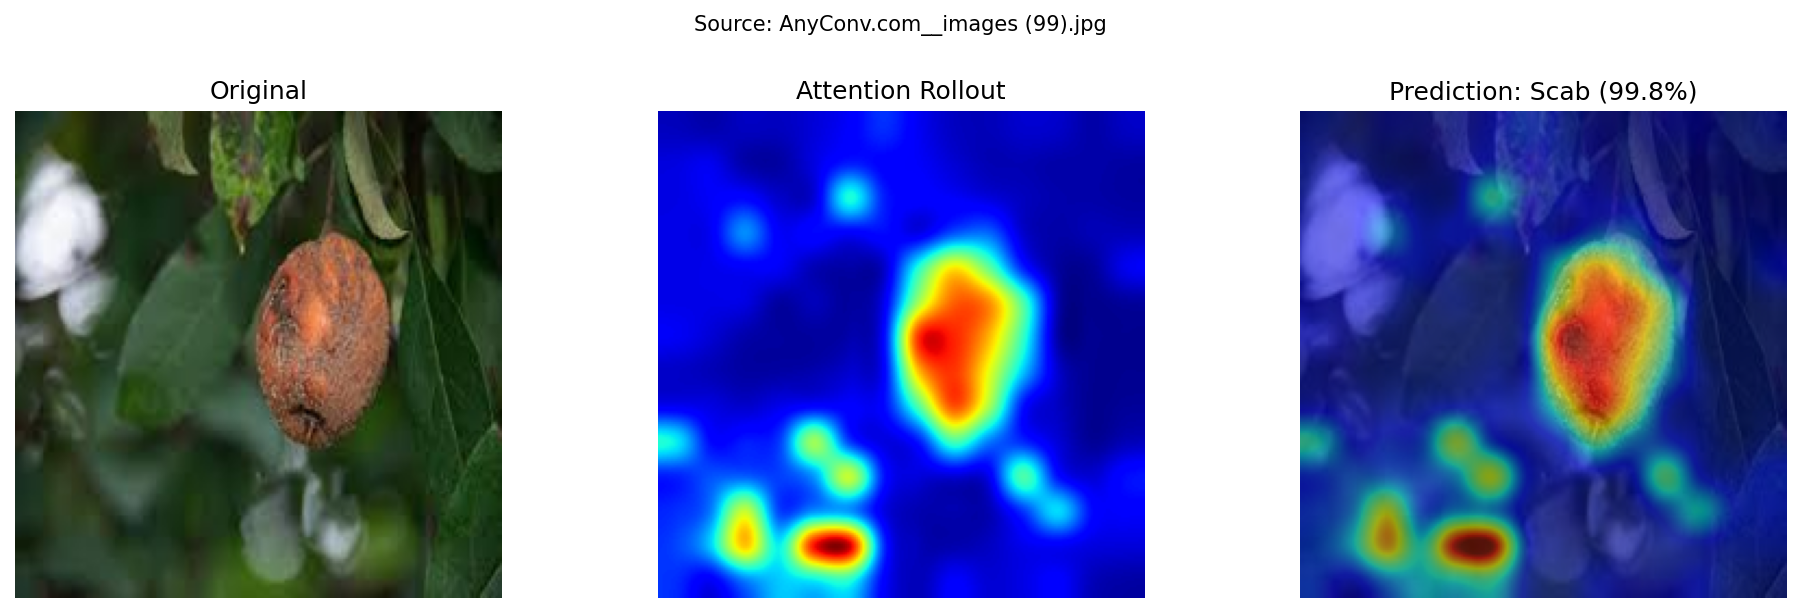
\includegraphics[width=0.95\textwidth]{attn_good_correct_33.png}
    \vspace{0.2em}
    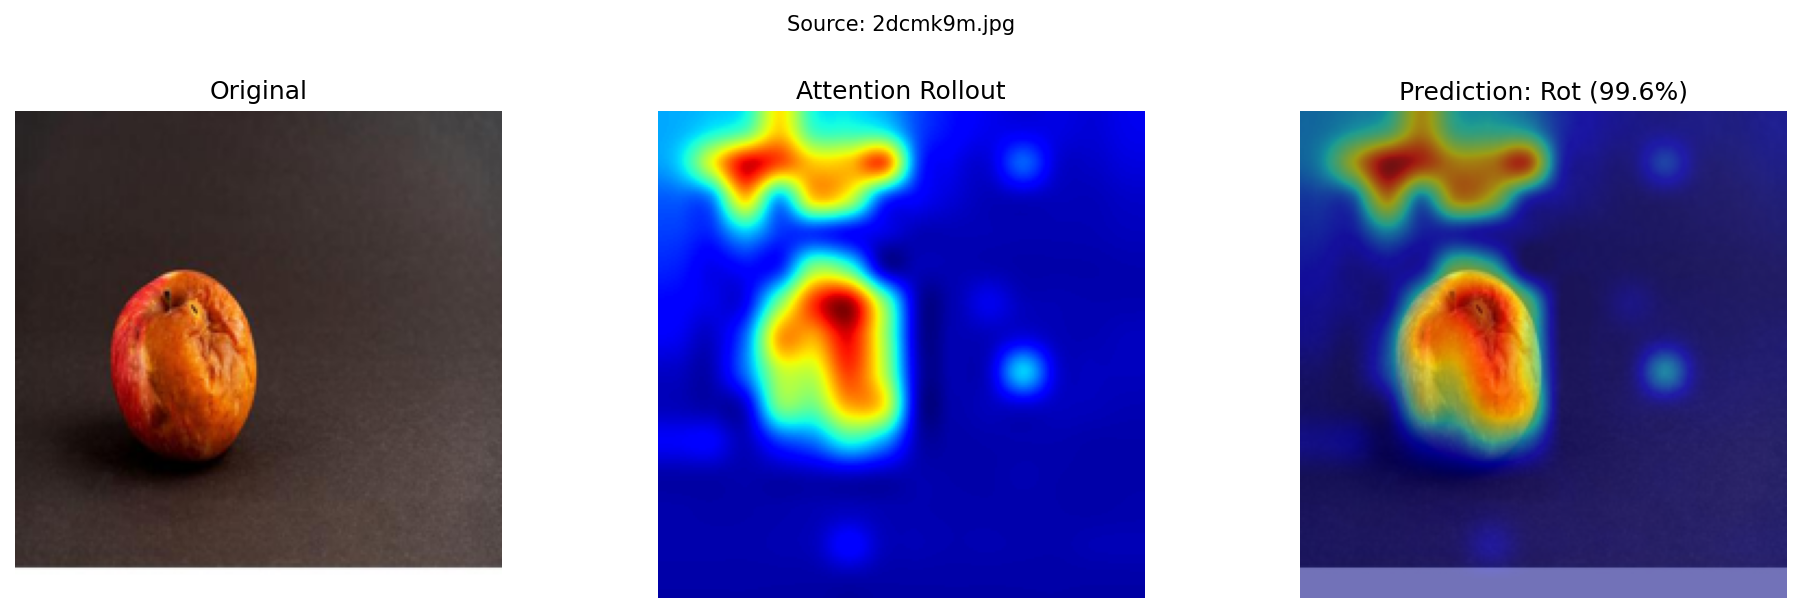
\includegraphics[width=0.95\textwidth]{attn_good_correct_54.png}
    \caption{Attention rollout examples (correct classifications). Each figure shows original image, attention heatmap, and overlay. These examples illustrate that the model can focus on the fruit region under varied backgrounds, though failure cases still exist and are under further analysis.}
\end{figure}

% =========================================================
\section*{6. Current Reservations and Questions}
% =========================================================
The baseline mIoU of 0.2682 quantitatively exposes the severe limitations of fixed-threshold HSV segmentation in real-world scenarios. As observed in our qualitative outputs (see Figure 1), the algorithm is highly susceptible to natural shadows and specular reflections on the waxy surface of the apples, leading to massive false positives. 

This obstacle validates our planned next steps: we must implement adaptive thresholding or watershed algorithms to improve the CV baseline's robustness against dynamic lighting. Furthermore, our initial ViT results indicate that the learning-based approach is promising on this dataset, motivating a deeper comparative analysis and interpretability study.

\vspace{0.5em}
\textbf{Gap analysis vs. proposal commitments (what remains):}
\begin{itemize}[noitemsep, topsep=0pt]
    \item \textbf{Attention map visualization (maximum goal):} Completed (initial). Next, we will expand qualitative analysis by grouping failure cases (shadow/specular highlight, texture confusion) and summarizing patterns.
    \item \textbf{Traditional CV robustness improvements:} Completed (initial). We implemented two robustness-motivated variants (adaptive thresholding on the V channel with CLAHE; and a watershed refinement). On our annotated subset, these initial variants did not outperform the fixed HSV baseline, highlighting the difficulty of tuning rule-based segmentation under diverse lighting.
    \item \textbf{Unified grading logic (maximum goal):} The proposal described a grading system (Premium / Grade I / Reject) integrating outputs from both pipelines (defect area ratio + class prediction). This integration and its quantitative evaluation are not yet completed.
    \item \textbf{Comprehensive comparative study:} We have initial results for both pipelines, but we still need a systematic comparison (e.g., per-class error analysis, qualitative failure cases, and ablations such as augmentation strength and sampler/class-weight toggles).
    \item \textbf{External validity / robustness checks (optional stretch):} Evaluate on additional data or controlled perturbations (lighting changes, blur, color shifts) to stress-test the CV baseline and the ViT model.
\end{itemize}

\vspace{0.5em}
\textbf{CV baseline robustness attempt (completed):} We benchmarked three traditional CV segmentation variants on the manually annotated subset (\texttt{mark\_pic/}; 40 image-mask pairs):
\begin{itemize}[noitemsep, topsep=0pt]
    \item \textbf{HSV fixed-threshold + morphology (baseline):} mean IoU = \textbf{0.2802}
    \item \textbf{Adaptive V-threshold (CLAHE + local/global threshold) + morphology:} mean IoU = 0.1048
    \item \textbf{Watershed refinement (built on adaptive mask):} mean IoU = 0.0915
\end{itemize}

\begin{figure}[h]
    \centering
    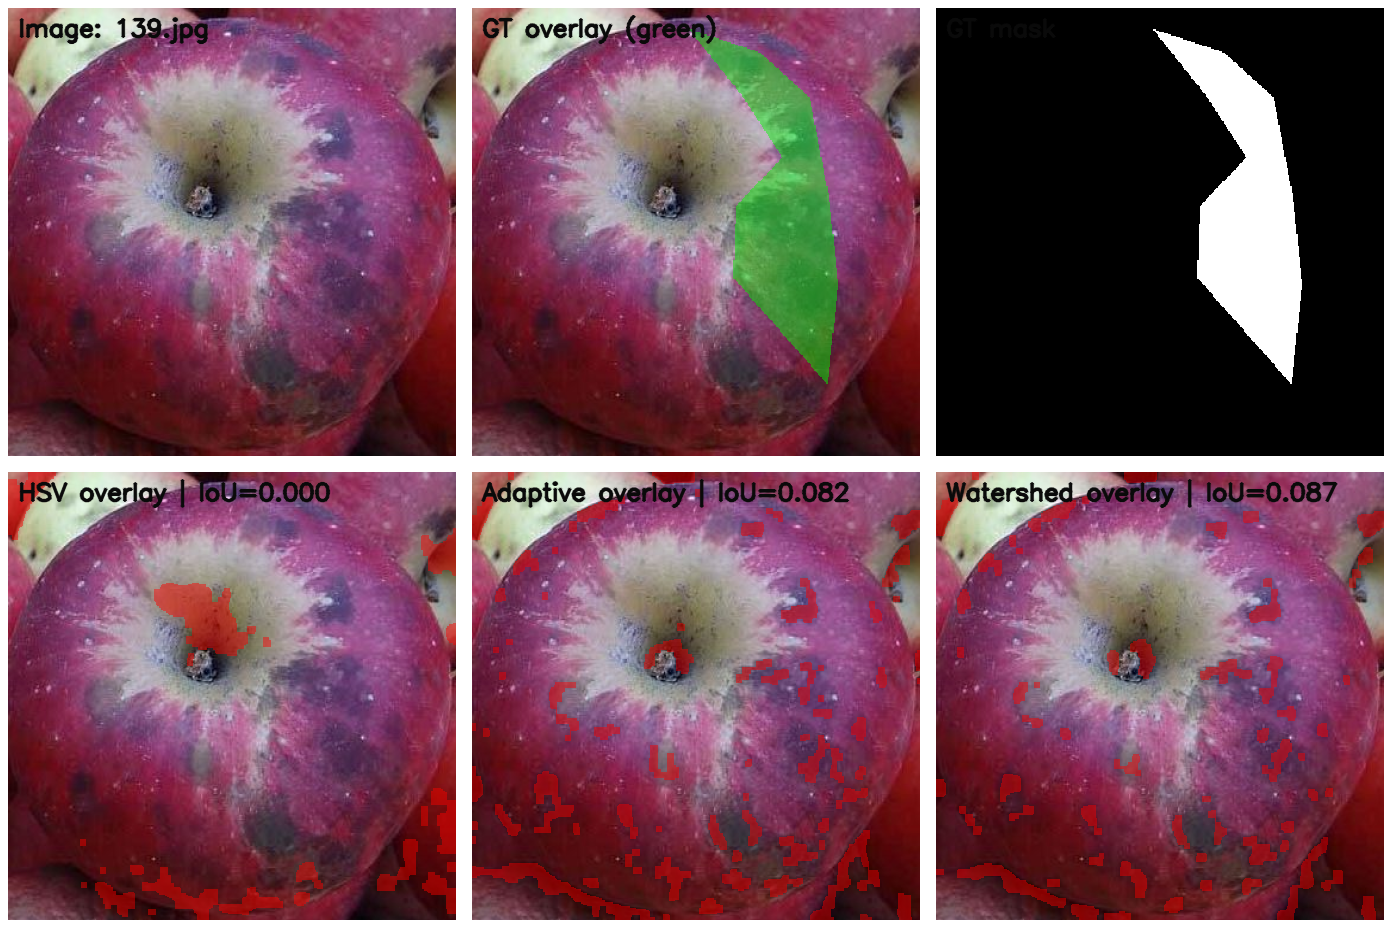
\includegraphics[width=0.98\textwidth]{cv_case_hard_1.png}
    \caption{Qualitative comparison on a challenging sample (overlay panels). Top row: image, GT overlay/mask. Bottom row: HSV baseline, adaptive, and watershed predictions with their IoU scores.}
\end{figure}

\begin{figure}[h]
    \centering
    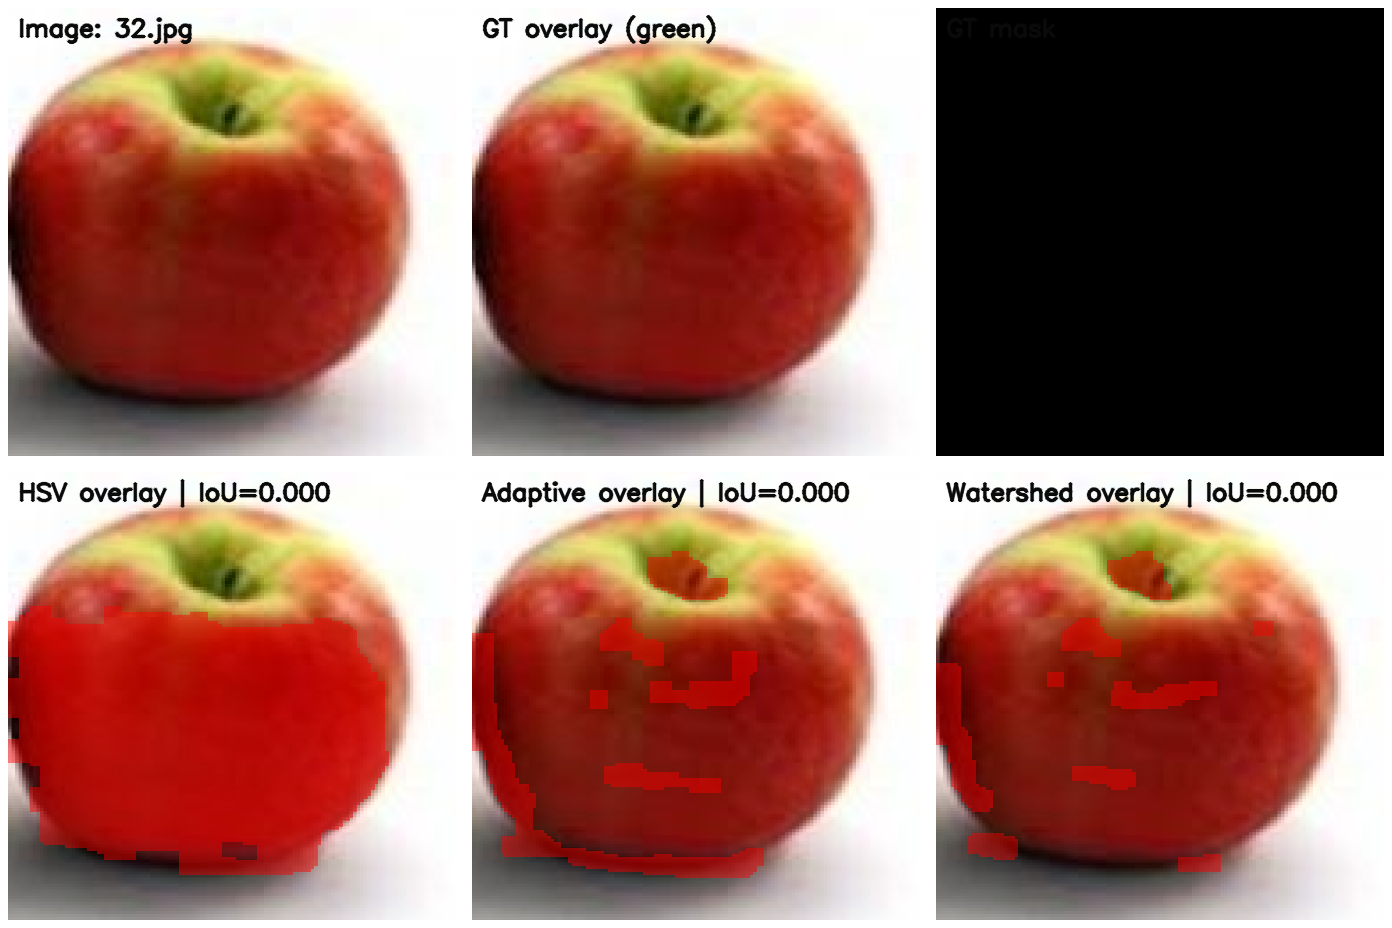
\includegraphics[width=0.98\textwidth]{cv_case_hard_2.png}
    \caption{Second qualitative comparison example for the CV segmentation variants.}
\end{figure}

% =========================================================
\section*{7. References}
% =========================================================
\begin{enumerate}[label={[\arabic*]}, noitemsep, topsep=0pt]
    \item Bradski, G. (2000). \textit{The OpenCV Library}. Dr. Dobb's Journal of Software Tools.
    
    \item Dosovitskiy, A., et al. (2020). \textit{An Image is Worth 16x16 Words: Transformers for Image Recognition at Scale}. ICLR 2021.

    \item Abnar, S., \& Zuidema, W. (2020). \textit{Quantifying Attention Flow in Transformers}. ACL 2020.

    \item Kaggle. \textit{Apple Fruit Disease Dataset}. Available at: \href{https://www.kaggle.com/datasets/kaivalyashah/apple-disease-detection}{https://www.kaggle.com/datasets/kaivalyashah/apple-disease-detection}.
\end{enumerate}

\end{document}